% vim: ts=2 sts=2 sw=2

\documentclass[a4paper,12pt]{report}
\usepackage{a4wide}
\usepackage[finnish]{babel}
\usepackage[utf8]{inputenc}
\usepackage[T1]{fontenc}
\usepackage{graphicx}
\usepackage{float}

\title{
\includegraphics[width=5em]{logo}\\\vspace{1em}MusicGhost\\\vspace{1em}
  \large{Tietokantasovellus, kevät 2011\\Tietojenkäsittelytieteen
  laitos\\Helsingin yliopisto}\\}
\author{Tuomo Lempiäinen\\\texttt{tuomo.lempiainen@helsinki.fi} \and
Hanna Nieminen\\\texttt{hanna.m.nieminen@helsinki.fi}}

\begin{document}

\maketitle

\tableofcontents

\chapter{Määrittely}

\section{Johdanto}

\subsection{Järjestelmän tarkoitus}

Järjestelmän avulla sen ylläpitäjä voi pitää kirjaa levykokoelmastaan.
Järjestelmä tarjoaa useita erillisiä listoja, jolloin on mahdollista
erotella esimerkiksi omistamansa levyt ja tulevat hankinnat toisistaan.
Järjestelmästä voi tehdä julkisen, jolloin myös vierailijat voivat selata
levylistaa ja yksittäisten levyjen tietoja.

\subsection{Toimintaympäristö}

Järjestelmää käytetään WWW-selaimen kautta. Sen ajamiseen tarvitaan
Apache-palvelin varustettuna PHP5-tuella sekä PostgreSQL-tietokanta.

\subsection{Rajaukset}

Kaikki ominaisuudet, joita ei ole tässä määrittelyssä erikseen mainittu, on
oletusarvoisesti rajattu järjestelmän ulkopuolelle.

\subsection{Toteutusympäristö}

Järjestelmän toteuttamisessa hyödynnetään Vim-editoria Arch Linux
-käyttöjärjestelmässä sekä Notepad++-editoria Windows 7
-käyttöjärjestelmässä. Toteutuksen aikana järjestelmää testataan
paikallisilla Apache- ja PostgreSQL-palvelimilla.

\section{Yleiskuva järjestelmästä}

\subsection{Sidosryhmäkaavio}

\vspace{1em}
\begin{figure}[H]
  \begin{center}
    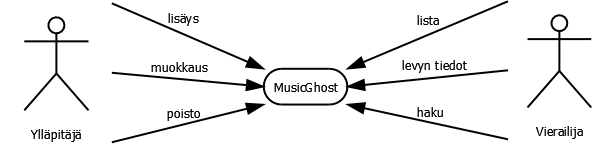
\includegraphics[width=\textwidth]{diagrams/sidosryhmakaavio}
  \end{center}
  \caption{Sidosryhmäkaavio}
\end{figure}

\subsection{Käyttäjäryhmät}

\begin{description}
  \item[Ylläpitäjä] Levytietokannan omistaja, joka ylläpitää tietokantaa.
  \item[Vierailija] Kuka tahansa sivulla vieraileva käyttäjä. Myös
    tietokannan omistaja kuuluu tähän luokkaan.
\end{description}

\section{Käyttötapaukset}

\subsection{Ylläpitäjä}

\begin{description}
  \item[Levyn lisääminen] Ylläpitäjä voi lisätä uusia levyjä tietokantaan.
    Ylläpitäjä syöttää ainakin levyn esittäjän, nimen, tyypin
    (albumi/single/\ldots) ja mahdollisen kokonaisuuden (boksin), johon levy
    kuuluu, sekä valitsee ainakin yhden listan, jolle se lisätään.
    Vapaaehtoisia tietoja ovat levyn julkaisuvuosi, formaatti, kotelointi,
    levy-yhtiö, painoksen koko, hankintapäivämäärä, tieto levyn lainassa
    olemisesta, vapaamuotoinen kommentti ja kansikuva.
  \item[Levyn tietojen muokkaaminen] Ylläpitäjä voi muokata kaikkia
    yksittäiseen levyyn liitettyjä tietoja.
  \item[Levyn poistaminen] Ylläpitäjä voi poistaa levyn tietokannasta.
  \item[Kirjautuminen ulos] Ylläpitäjä voi tarvittavat ylläpitotehtävät
    tehtyään kirjautua ulos, jolloin hänestä tulee tavallinen vierailija.
\end{description}

\subsection{Vierailija}

\begin{description}
  \item[Levylistan selaaminen] Kuka tahansa voi katsella tietokannan
    sisältöä.  Listauksessa näkyy kunkin levyn kohdalla sen esittäjä, nimi,
    julkaisuvuosi ja formaatti.
  \item[Yksittäisen levyn tietojen tutkiminen] Käyttäjä voi valita
    yksittäisen levyn, jolloin hänelle näytetään kaikki siihen liitetyt
    tiedot.
  \item[Levyjen hakeminen hakusanalla] Käyttäjä voi antaa hakusanoja,
    jolloin hänelle näytetään lista niistä levyistä, joiden listauksessa
    näytettävät tiedot sisältävät annetut hakusanat.
  \item[Kirjautuminen sisään] Mikäli vierailija tietää ylläpitäjän
    salasanan, hän voi kirjautua sisään järjestelmään, jolloin hänestä tulee
    ylläpitäjä.
\end{description}

\chapter{Suunnittelu}

\section{Järjestelmän tietosisältö}

\begin{figure}[H]
  \begin{center}
    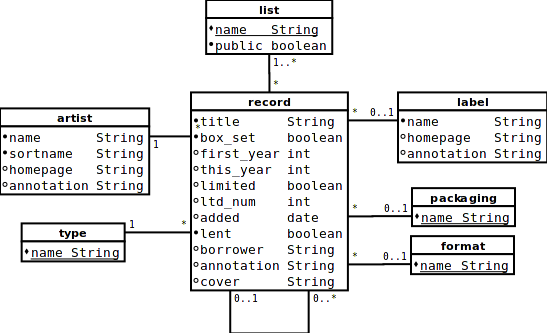
\includegraphics[width=0.8\textwidth]{diagrams/kasitekaavio}
  \end{center}
  \caption{Käsitekaavio}
\end{figure}

\begin{description}

  \item[artist]
    Levyn esittäjä identifioidaan yksikäsitteisen kokonaisluku-id:n avulla.
    Esittäjä voi liittyä tietokannassa mielivaltaiseen määrään levyjä.
    \begin{description}
      \item[name] Esittäjän nimi (esimerkiksi ''Etunimi Sukunimi'')
      \item[sortname] Nimi, jota käytetään esittäjien järjestämiseen
        (esimerkiksi ''Sukunimi, Etunimi'')
      \item[homepage] Esittäjän kotisivujen osoite
      \item[annotation] Vapaamuotoinen kuvaus esittäjästä
    \end{description}

  \item[label]
    Levy-yhtiö identifioidaan yksikäsitteisen kokonaisluku-id:n avulla.
    Levy-yhtiö voi liittyä tietokannassa mielivaltaiseen määrään levyjä.
    \begin{description}
      \item[name] Levy-yhtiön nimi
      \item[homepage] Levy-yhtiön kotisivujen osoite
      \item[annotation] Vapaamuotoinen kuvaus levy-yhtiöstä
    \end{description}

  \item[record]
    Omistajan levykokoelmaan kuuluva levy. Levy identifioidaan
    yksikäsitteisen kokonaisluku-id:n avulla.  Levyyn liittyy sen esittäjä
    ja tyyppi. Siihen voi liittyä myös enintään yksi levy-yhtiö, formaatti
    ja kotelon tyyppi.  Lisäksi levy kuuluu ainakin yhteen listaan. Levy voi
    kuulua samaan boksiin joidenkin muiden levyjen kanssa.
    \begin{description}
      \item[title] Levyn nimi (merkkijono)
      \item[box\_set] Onko kyseessä boksi, johon voi sisältyä muita levyjä?
        (totuusarvo)
      \item[first\_year] Levyn alkuperäinen julkaisuvuosi (kokonaisluku)
      \item[this\_year] Kokoelmassa olevan version julkaisuvuosi (kokonaisluku)
      \item[limited] Onko levy rajoitettua painosta? (totuusarvo)
      \item[ltd\_num] Rajoitetun painoksen painosmäärä (kokonaisluku)
      \item[added] Päivä, jolloin levy on lisätty kokoelmaan (päivämäärä)
      \item[lent] Onko levy lainassa? (totuusarvo)
      \item[borrower] Henkilö, jolle levy on lainattu (merkkijono)
      \item[annotation] Vapaamuotoinen kuvaus levystä (merkkijono)
      \item[cover] Levyn kansikuvan tiedostonnimi (merkkijono)
    \end{description}

  \item[type]
    Levytyyppi voi liittyä tietokannassa mielivaltaiseen määrään levyjä.
    \begin{description}
      \item[name] Levyn tyyppi, esimerkiksi ''Album'' tai ''Single''
        (merkkijono)
    \end{description}

  \item[format]
    Levyformaatti voi liittyä tietokannassa mielivaltaiseen määrään levyjä.
    \begin{description}
      \item[name] Levyn formaatti, esimerkiksi ''2CD'' tai ''DVD+CD''
        (merkkijono)
    \end{description}

  \item[packaging]
    Kotelotyyppi voi liittyä tietokannassa mielivaltaiseen määrään levyjä.
    \begin{description}
      \item[name] Levyn kotelon tyyppi, esimerkiksi ''Jewel case'' tai
        ''Digipak'' (merkkijono)
    \end{description}

  \item[list]
    Levylista, johon voi liittyä mielivaltainen määrä levyjä.
    Lista identifioidaan sen yksikäsitteisen nimen perusteella.
    \begin{description}
      \item[name] Listan nimi (merkkijono)
      \item[public] Onko lista julkinen? (totuusarvo)
      \item[default] Onko kyseeessä oletuslista, joita on vain yksi?
        (totuusarvo)
    \end{description}

\end{description}

\section{Käyttöliittymän hahmotelma}

\begin{figure}[H]
  \begin{center}
    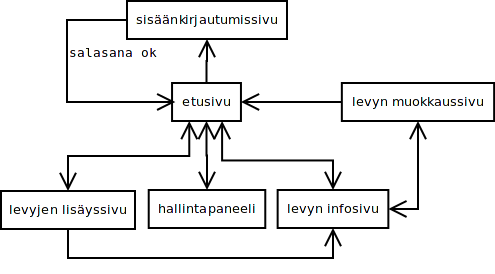
\includegraphics[width=0.8\textwidth]{diagrams/kalikaavio}
  \end{center}
  \caption{Sivujen välillä liikkuminen}
\end{figure}

\begin{figure}[H]
  \begin{center}
    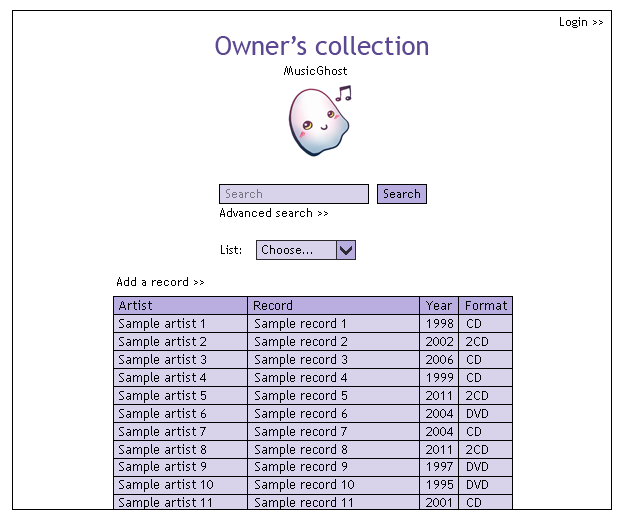
\includegraphics[width=\textwidth]{uidraft/mainwindow2}
  \end{center}
  \caption{Etusivu}
\end{figure}

\begin{figure}[H]
  \begin{center}
    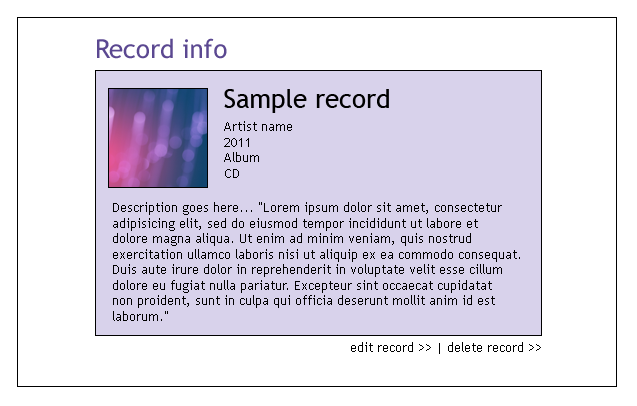
\includegraphics[width=\textwidth]{uidraft/recordinfopage}
  \end{center}
  \caption{Levyn lisätietosivu}
\end{figure}

\begin{figure}[H]
  \begin{center}
    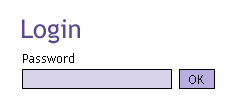
\includegraphics[]{uidraft/login}
  \end{center}
  \caption{Sisäänkirjautumissivu}
\end{figure}

\begin{figure}[H]
  \begin{center}
    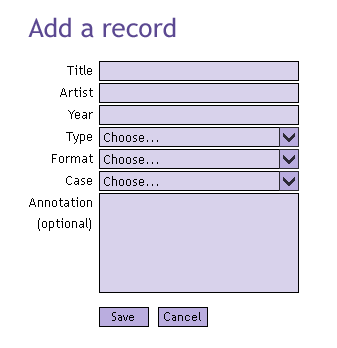
\includegraphics[]{uidraft/addpage}
  \end{center}
  \caption{Levyn lisäyssivu}
\end{figure}

\begin{figure}[H]
  \begin{center}
    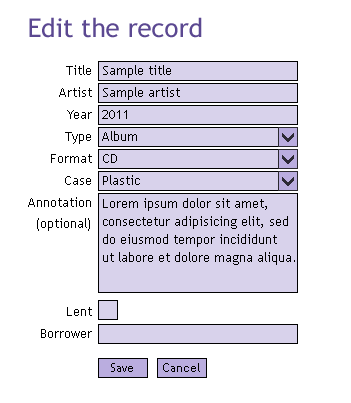
\includegraphics[]{uidraft/editpage}
  \end{center}
  \caption{Levyn muokkaussivu}
\end{figure}

\begin{figure}[H]
  \begin{center}
    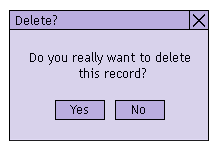
\includegraphics[]{uidraft/delete}
  \end{center}
  \caption{Levyn poiston varmistusdialogi}
\end{figure}

\section{Relaatiotietokantakaavio}

Relaatiotietokantakaavio on esitetty \texttt{CREATE TABLE} -lauseina
tiedostossa \texttt{sql/init\_db.sql}.

Käsitemalliin nähden relaatiotietokantakaavioon on lisätty tunnistavat
id-sarakkeet niille kohteille, joille ei käsitemallissa ollut tunnistavia
attribuutteja. Tietokohteiden välisiä yhteyksiä varten on myös lisätty
sarakkeet. Kohteiden record ja list välinen monen suhde moneen -yhteys on
toteutettu lisäämällä uusi taulu record\_list.

\chapter{Toteutus}

\section{Johdanto}

\subsection{Järjestelmän tarkoitus}

Järjestelmän avulla sen ylläpitäjä voi pitää kirjaa levykokoelmastaan.
Järjestelmä tarjoaa useita erillisiä listoja, jolloin on mahdollista
erotella esimerkiksi omistamansa levyt ja tulevat hankinnat toisistaan.
Järjestelmästä voi tehdä julkisen, jolloin myös vierailijat voivat selata
levylistaa ja yksittäisten levyjen tietoja.

\subsection{Toimintaympäristö}

Järjestelmää käytetään WWW-selaimen kautta. Sen ajamiseen tarvitaan
Apache-palvelin varustettuna PHP5-tuella sekä PostgreSQL-tietokanta.

\subsection{Rajaukset}

Kaikki ominaisuudet, joita ei ole tässä määrittelyssä erikseen mainittu, on
oletusarvoisesti rajattu järjestelmän ulkopuolelle.

\subsection{Toteutusympäristö}

Järjestelmän toteuttamisessa hyödynnettiin Vim-editoria Arch Linux
-käyttöjärjestelmässä sekä Notepad++-editoria Windows 7
-käyttöjärjestelmässä. Toteutuksen aikana järjestelmää testattiin
paikallisilla Apache- ja PostgreSQL-palvelimilla.

\section{Ohjelmiston yleisrakenne}

\begin{figure}[H]
  \begin{center}
    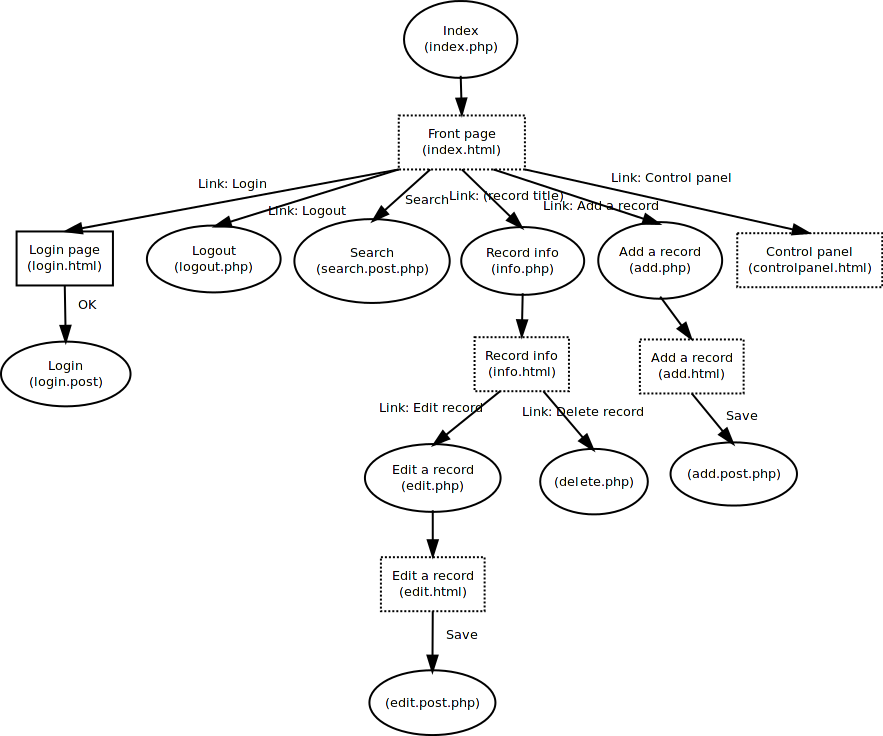
\includegraphics[width=\textwidth]{diagrams/rakennekaavio}
  \end{center}
  \caption{Rakennekaavio}
\end{figure}

\section{Järjestelmän komponentit}

\subsection{Näkymät}

\subsubsection{Etusivu}

Generoitu html-sivu, jonka tuottaa toiminto front.php. Kuva näkymästä
liitteenä X.

Sivuun liittyvät tiedostot:
\begin{itemize}
  \item logo.png: levytietokannan logo
\end{itemize}

Etusivulla on tiivis listaus käyttäjän tietokannassa olevista levyistä
(levyistä näytetään niiden esittäjä, nimi, julkaisuvuosi ja formaatti) sekä
alasvetovalikko ja hakukenttä, joiden avulla voidaan tarkastella eri
listoille luokiteltuja levyjä jonkin suodattimen kanssa.  Hakukentän
käsittelee toiminto front.post.php, joka käynnistetään Show-nappia
painamalla.  Tietokannan levyjen listauksessa jokaisen levyn nimi toimii
linkkinä kyseisen levyn infosivulle.

Lisäksi sivulla on seuraavat linkit:

\begin{itemize}
  \item Sisäänkirjautumattomalle käyttäjälle:
    \begin{itemize}
	    \item Login (kirjaudu sisään),
		    vie sisäänkirjautumissivulle
    \end{itemize}

  \item Sisäänkirjautuneelle käyttäjälle:
    \begin{itemize}
	    \item Logout (kirjaudu ulos),
		    kirjaa käyttäjän ulos
	    \item Add a record (lisää levy),
		    vie levyn lisäyssivulle
	    \item Control panel (hallintapaneeli),
		    vie tietokannan hallintapaneelisivulle
    \end{itemize}
\end{itemize}

\subsubsection{Sisäänkirjautumissivu}

Generoitu html-sivu. Kuva näkymästä liitteenä X.

Sivulla on kenttä salasanan kirjoittamista varten sekä OK-painike.
Painiketta painettaessa toiminto login.post.php käsittelee lomakkeen.  Isoja
ja pieniä kirjaimia ei tulkita samoiksi.

\subsubsection{Levyjen lisäys- ja muokkaussivut}

Generoidut html-sivut, jotka tuottaa toiminto addedit.php. Kuvat näkymistä
liitteinä X ja Y.

Kummallakin sivulla on lomake, jossa on kentät Artist (esittäjä), Title
(levyn nimi), Box set (onko levy normaali, boksi vai boksiin kuuluva levy),
Type (tyyppi), Year (first release) (ensimmäisen julkaisun vuosi), Year
(this release) (kokoelmassa olevan levyn julkaisuvuosi), Format (formaatti),
Packaging (kotelon tyyppi), Label (levy-yhtiö), Limited (rajoitettu painos,
rajoitetun painoksen painosmäärä), Added (lisäämispäivämäärä), Lent (onko
levy lainassa ja lainaajan nimi) ja Annotation (kuvaus levystä) sekä Cover
(kansikuva) -tiedostonlähetyskenttä, jonka avulla voidaan ladata omalta
tietokoneelta kansikuva palvelimelle.

Muokkaussivulla lomake on täytetty valmiiksi tietokannasta löytyvillä
vanhoilla tiedoilla.

Lomakkeen tiedot lähettää nappi Save ja tyhjentää nappi Reset. Save-napin
painamisen jälkeen lomakkeen käsittelee toiminto addedit.post.php.

Sivulla on lisäksi linkki Front page, joka vie takaisin etusivulle.

\subsubsection{Levyn infosivu}

Generoitu html-sivu, jonka tuottaa toiminto details.php. Kuvanäkymästä
liitteenä X.

Sivuun liittyvät tiedostot:
\begin{itemize}
  \item levyn kansikuva, mikäli sellainen on talletettu tietokantaan
\end{itemize}

Sivulla on levyn kansikuva (jos sellainen löytyy tietokannasta) sekä levyn
esittän, levyn ja levy-yhtiön tietokannasta löytyvät tiedot (esittäjän nimi,
esittäjän kotisivu, kuvaus esittäjästä, levyn julkaisuvuodet - alkuperäinen
ja kokoelmassa olevan levyn julkaisuvuosi, tyyppi, formaatti, kotelon
tyyppi, rajoitetun painoksen tapauksessa painosmäärä, lisäyspäivämäärä,
tieto siitä, onko levy lainattu ja kenelle, kuvaus levystä, levy-yhtiön
nimi, levy-yhtiön kotisivu ja kuvaus levy-yhtiöstä).

Sivulla on linkki Front page, joka vie takaisin etusivulle.
Sisäänkirjautuneelle käyttäjälle näytetään lisäksi linkit:

\begin{itemize}
  \item Edit record (muokkaa levyä),
		vie levyn muokkausssivulle
  \item Delete record (poista levy).  Varmistaa
    JavaScript-ilmoitusikkunassa, haluaako käyttäjä todella poistaa levyn.
    Jos käyttäjä klikkaa OK-painiketta, toiminto delete.php poistaa levyn
    tietokannasta ja ohjaa käyttäjän sen jälkeen etusivulle.
    Cancel-painikkeen klikkaaminen ei aiheuta muutoksia.
\end{itemize}

Lisäksi sivulla on em. linkit esittäjän ja levy-yhtiön kotisivuille, mikäli
ne on talletettu tietokantaan.

\subsubsection{Levytietokannan hallintapaneeli}

Generoitu html-sivu, jonka tuottaa toiminto control.php. Kuva näkymästä
liitteenä X.

Sivulla on välilehdet Artists (esittäjät) ja Labels (levy-yhtiöt), joilla
voi lisätä, muokata ja poistaa tietokannasta löytyviä esittäjiä ja
levy-yhtiöitä.

Artists-välilehdellä on alasvetovalikko, josta voi valita, lisääkö uuden
esittäjän vai muokkaako jotain tietokannasta ennestään löytyvää esittäjää.
Valinta varmistetaan painamalla painiketta Show, jolloin toiminnot
control.php ja control.post.php käsittelevät tapahtuman.  Välilehdellä on
kentät Name (nimi), Sortname (esittäjien järjestämiseen käytettävä nimi),
Homepage (kotisivu) ja Annotation (vapaavalintainen kuvaus esittäjästä). Jos
muokataan tietokannasta vanhastaan löytyvää artistia, lomake on esitäytetty
tietokannasta löytyvillä tiedoilla.  Lomakkeen tiedot tallennetaan
Save-nappia painamalla tai valittu esittäjä poistetaan tietokannasta
Delete-nappia painamalla.  Nappia painettaessa toiminnot control.php ja
control.post.php käsittelevät tapahtuman.

Labels-välilehti on täysin vastaavanlainen (lukuunottamatta
Sortname-kenttää, jota ei ole).

Lisäksi sivulla on linkki Front page, joka vie takaisin etusivulle.

\subsection{Toiminnot}

\subsubsection{front.php}

Toiminto auttaa generoimaan tietokantasovelluksen etusivunäkymän.
Käynnistyksen yhteydessä ei välitetä parametreja.

Toiminto tekee tietokantakyselyt, joilla haetaan taulusta list
sisäänkirjautuneen käyttäjän tapauksessa kaikki listat ja
sisäänkirjautumattoman käyttäjän tapauksessa vain julkiset listat.  Toiminto
hakee myös tarvittaessa tietokannasta ne levyt, joissa esiintyy tietty
suodatinsana.  Lisäksi haetaan taulusta record jokaisen levyn id, nimi,
alkuperäinen julkaisuvuosi ja formaatti sekä taulusta artist levyn esittäjän
nimi. Toiminto myös generoi jokaista levyä vastaavan infosivun urlin.

\subsubsection{login.post.php}

Toiminto käynnistetään sisäänkirjautumissivulta käsittelemään
kirjautumislomake. Toiminto tarkistaa käyttäjän käyttöoikeuden tämän
syöttämän salasanan perusteella.  Jos annettu salasana on oikea, laitetaan
Atomikin session päälle ja generoidaan etusivu, jolla näkyy myös ylläpitoon
tarvittavat linkit. Jos salasana on väärä, ei tehdä mitään.

Toiminnon parametrit:
\begin{itemize}
  \item password (salasana): merkkijono
\end{itemize}

\subsubsection{logout.php}

Toiminto käynnistetään etusivulta linkkiä Logout klikkaamalla. Toiminto
kirjaa käyttäjän ulos (Atomikin session) ja ohjaa käyttäjän takaisin
etusivulle.

\subsubsection{addedit.php}

Toiminto auttaa generoimaan levyjen lisäys- ja muokkaussivut. Käynnistyksen
yhteydessä ei välitetä parametreja.  Toiminto käynnistyy etusivulta linkkiä
Add a record klikkaamalla tai levyn infosivulta linkkiä Edit record
klikkaamalla.

Toiminto tarkistaa ensin, onko käyttäjä kirjautunut sisään.  Sen jälkeen
tehdään tietokantakyselyt, joilla haetaan kaikkien esittäjien id:t taulusta
artist (ja järjestetään ne sortnamen mukaan), kaikki eri boxset-tyypit,
kaikki levytyypit taulusta type, kaikki formaatit taulusta format, kaikki
kotelotyypit taulusta packaging ja kaikki levy-yhtiöiden id:t taulusta label
(ja järjestetään ne nimen mukaan).

\subsubsection{addedit.post.php}

Toiminto käynnistetään levyjen lisäämisnäkymästä käsittelemään lisäyslomake
tai levyn muokkausnäkymästä käsittelemään muokkauslomake.  Toiminto
tarkistaa käyttäjän lomakkeelle syöttämät tiedot ja antaa tarvittaessa
virheilmoituksen puuttuvista pakollisista tiedoista.  Kelvolliset parametrit
saatuaan ohjelma lisää tauluun record käyttäjän haluaman levyn tai päivittää
muokattavan levyn tiedot taulussa record.

Toiminnon parametrit:
\begin{itemize}
  \item artist (esittäjä): kokonaisluku (id jollekin tietokannasta
    löytyvälle esittäjälle, jotka on lueteltu alasvetovalikossa)
  \item title (levyn nimi): merkkijono
  \item boxset (onko levy normaali, boksi vai boksiin kuuluva levy):
    merkkijono (normal, boxset tai item)
  \item box\_id (boksin tunniste): kokonaisluku
  \item type (tyyppi): merkkijono (album, single, EP, compilation,
    soundtrack, interview, live tai other)
  \item year (first release) (ensimmäisen julkaisun vuosi): kokonaisluku
  \item year (this release) (kokoelmassa olevan levyn julkaisuvuosi):
    kokonaisluku
  \item format (formaatti): merkkijono (CD, 2CD, DVD, CD+DVD, DVD+CD)
  \item packaging (kotelon tyyppi): merkkijono (jewel case, digipack, keep
    case tai other)
  \item label (levy-yhtiö): kokonaisluku (id jollekin levy-yhtiölle, jotka
    on lueteltu alasvetovalikossa)
  \item limited (onko rajoitettu painos): boolean
  \item ltd\_num (rajoitetun painoksen painosmäärä): kokonaisluku
  \item added (lisäyspäivämäärä): date
  \item lent (onko levy lainassa): boolean
  \item borrower (lainaajan nimi): merkkijono
  \item annotation (kuvaus levystä): merkkijono
  \item cover (kansikuvan tiedostonimi): merkkijono
\end{itemize}

\subsubsection{details.php}

Toiminto käynnistetään etusivulta klikkaamalla jonkin levyn nimeä, jolloin
se auttaa generoimaan levyn lisätietosivun.  Toiminto saa parametrinaan
levyn id:n.

Toiminto tekee tietokantakyselyn, jolla haetaan taulusta record levyn tiedot
(nimi, onko se osa boksia, boksin tunniste, tyyppi, julkaisuvuodet,
formaatti, kotelon tyyppi, onko rajoitettu painos, rajoitetun painoksen
numero, lisäyspäivämäärä, onko lainattu, lainaajan nimi, levyn kuvaus,
kansikuva), taulusta artist levyn esittäjän nimi, kotisivu ja kuvaus sekä
taulusta label levy-yhtiön nimi, kotisivu ja kuvaus.

\subsubsection{delete.php}

Toiminto käynnistetään levyn infosivulta klikkaamalla Delete record -linkkiä
ja valitsemalla ilmestyvästä varmistusikkunasta OK-painike. Toiminnon
parametrina välitetään poistettavan levyn id.

Toiminto tarkistaa ensin, onko käyttäjä kirjautunut sisään, poistaa sitten
levyn tietokannasta ja ohjaa käyttäjän takaisin etusivulle.

\subsubsection{control.php}

Toiminto käynnistetään etusivulta klikkaamalla linkkiä Control panel, ja se
auttaa generoimaan levytietokannan hallintapaneelin välilehtineen.

Toiminto tarkistaa ensin, onko käyttäjä kirjautunut sisään. Tietokannasta
haetaan kaikki esittäjät ja levy-yhtiöt.

\subsubsection{control.post.php}

Toiminto käynnistetään käsittelemään lomake, kun hallintapaneelissa
klikataan Show-, Save- tai Delete-painiketta.  Show-napin tapauksessa
valinnasta riippuen toiminto joko generoi tyhjän lomakkeen tai hakee
tietokannasta valitun esittäjän tai levy-yhtiön tiedot lomaketta varten.
Save-nappia painettaessa toiminto tarkistaa käyttäjän syöttämät tiedot,
generoi tarvittaessa virheilmoitukset ja kelvolliset tiedot saatuaan lisää
esittäjän tai levy-yhtiön tietokantaan tai päivittää vanhat tiedot.
Delete-nappia painettassa toiminto tarkistaa, onko esittäjällä tai
levy-yhtiöllä levyjä tietokannassa. Myönteisessä tapauksessa se generoi
virheilmoituksen, kielteisessä poistaa valitun esittäjän tai levy-yhtiön
tietokannasta.

Toiminnon parametrit:
\begin{itemize}
  \item entry (valitun esittäjän tai levy-yhtiön tunniste): kokonaisluku
  \item name (valitun esittäjän tai levy-yhtiön nimi): merkkijono
  \item sortname (valitun esittäjän järjestysnimi): merkkijono
  \item homepage (valitun esittäjän tai levy-yhtiön kotisivun url): merkkijono
  \item annotation (valitun esittäjän tai levy-yhtiön vapaavalintainen
    kuvaus): merkkijono
\end{itemize}

\subsection{Muut komponentit}

\begin{itemize}
  \item style.css: Sivujen ulkoasun määrittelevä css-tiedosto.
  \item logo.png: Levytietokannan logo.
  \item favicon.ico: Selaimen osoiterivillä näkyvä pikkukuvake.
  \item levyjen kansikuvat
\end{itemize}

\section{Asennustiedot}

\section{Käyttöohje}

\section{Liitteet}

\end{document}
